% !TEX encoding = UTF-8
% !TEX TS-program = pdflatex
% !TEX root = ../tesi.tex

%**************************************************************
\chapter{Progettazione e realizzazione} %TODO e codifica
\label{cap:progettazione}
%**************************************************************

\intro{Il capitolo corrente ha lo scopo di illustrare l'architettura del plugin nel  dettaglio con il supporto di diagrammi e le scelte progettuali effettuate.}\\

\section{Procedura di lavoro}
Inizialmente per capire il funzionamento di un plugin Maven e delle API RESTful del server documentale (Confluence), è stato dedicato del tempo allo studio autonomo.
Successivamente è stato sviluppato un Proof of Concept al fine di mettere in pratica quanto appreso dalla teoria.
Il prototipo consisteva in un semplice plugin Maven che effettuava delle stampe e delle chiamate REST ad un server creato al momento con Meecrowave.
Questo prototipo è successivamente cresciuto ed è stato ampliato e modificato per poter interagire con il plugin \emph{Docs} di Confluence.
Ciò ha permesso di comprendere il caricamento di materiale su \emph{Docs} ed ha consentito di effetture la scelta delle librerie Java più adatte per il prodotto finale.


%**************************************************************
\section{Tecnologie e librerie utilizzate}
\label{sec:tecnologie-strumenti}

In questa sezione viene data una panoramica delle tecnologie e librerie principali utilizzate.
Esse sono state scelte dalla candidata in concomitanza con gli sviluppatori DevOps senior dell'azienda.


\subsection{JavaX}
JavaX è un package di estensioni standard per il linguaggio Java.
Le estensioni che include sono numerose; quelle usate per la realizzazione del prodotto sono:
\begin{itemize}
    \item \bd{javax.annotation}: ovvero \emph{Java Null annotation}, per le annotazioni  \texttt{Nonnull} e  \texttt{Nullable}, richieste secondo la politica aziendale, in modo da segnalare gli elementi che possono essere nulli o meno;
    \item \bd{javax.ws.rs.core}: ovvero \emph{JAX-RS}, per la creazione di risorse relative ai servizi RESTful, utili per il client al momento della comunicazione con Confluence;
    % Low-level interfaces and annotations used to create RESTful service resources
    \item \bd{javax.xml.bind.annotation}: ovvero \emph{JAXB}, per la trasformazione automatica di JSON in oggetti Java, utile per convertire i messaggi mandati da Confluence in oggetti facilmente manipolabili dal plugin.
\end{itemize}


\subsection{Codehaus Plexus}
Codehaus Plexus è una collezione di componenti usata da Apache Maven.
Le librerie adottate per il progetto sono:
\begin{itemize}
    \item \bd{org.codehaus.plexus.archiver}: per l'archiviazione della documentazione;
    \item \bd{org.codehaus.plexus.util}: per utilità varie, adatte per la scrittura su file.
\end{itemize}


\subsection{Maven}
Maven è la tecnologia centrale del prodotto.
Di essa sono state utilizzate numerose classi, ma i package principali sono:
\begin{itemize}
    \item \bd{org.apache.maven.plugins.annotations}: per le annotazioni relative ai plugin Maven, quali per esempio \texttt{Mojo} per identificare un \emph{goal},  \texttt{Paremeter} per segnalare un parametro della configurazione, ecc;
    \item \bd{org.apache.maven.plugin}: per le eccezioni che può lanciare un plugin Maven;
    \item \bd{org.apache.maven.project}: per accedere alle informazioni del progetto (quali nome e versione);
    \item \bd{org.apache.maven.settings}: per decriptare le credenziali provenienti dal file ``settings.xml''.
\end{itemize}


\subsection{Jersey} %aveva tanta documentazione rispetto ad altri client
Jersey è un framework opensource per lo sviluppo di servizi web RESTful in Java.
All'interno del progetto è stata una parte focale perché utilizzato per la creazione del client:
\begin{itemize}
    \item \bd{com.sun.jersey.api.client}: per il client che effettua le chiamate verso Confluence;
    \item \bd{com.sun.jersey.api.client.config}: per la configurazione iniziale del client.
\end{itemize}



%**************************************************************
\section{Diagramma dei package} %TODO da rifare
\label{sec:diagramma-package}
\begin{figure}[H]
    \centering
    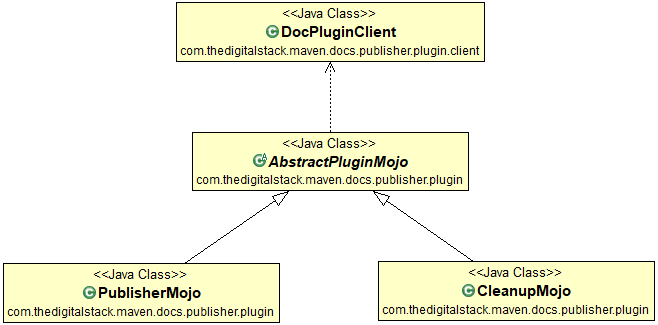
\includegraphics[width=0.8\textwidth]{immagini/PackageDiagram.png}\\
    \caption{Diagramma dei package}
\end{figure}
Le classi principali del \emph{Maven documentation publisher plug-in} sono i \emph{mojos} di Maven e il client.
Un \emph{mojo} è un \emph{goal} esguibile in Maven, ovvero la classe che concretamente realizza lo scopo prefissato.
I \emph{mojos} appartengono al package Java \texttt{com.thedigitalstack.maven.docs.publisher.plugin} e il client al sub-package\\ \texttt{com.thedigitalstack.maven.docs.publisher.plugin.client}.
Tra loro è possibile identificare due classi fondamentali: PublisherMojo e CleanupMojo.
Entrambe sono \emph{mojos} di Maven e perciò determinano \emph{goal} differenti.
Alcuni metodi che riguardano il client e le impostazioni del server sono uguali, per questo motivo esiste una classe padre e un riferimento a DocPluginClient.
DocPluginClient svolge le operazioni lato client ed è l'unico oggetto che comunica direttamente con Confluence.



%**************************************************************
\section{Diagrammi delle classi}
\label{sec:diagrammi-classi}

\begin{figure}[H]
    \centering
    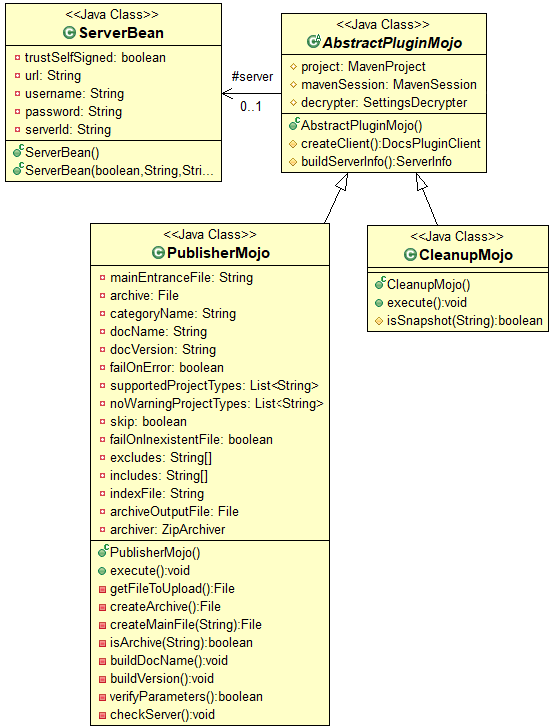
\includegraphics[width=0.95\textwidth]{immagini/mojo-gerarchy.png}\\
    \caption{Diagramma delle classi relativo alla gerarchia principale del plugin}
\end{figure}

\txt{PublisherMojo} realizza la pubblicazione della documentazione su Confluence, per questo motivo, il suo \emph{goal} è nominato \emph{publish} e la fase del ciclo di vita Maven relativo al progetto è package di default.

%TODO sistemare tabella con i parametri
\begin{table}[H]
    \centering
    {\def\arraystretch{1.7}
    \begin{tabularx}{\textwidth}{XXXX}
        \rowcolor{beautyblue} \textbf{Parametro} & \textbf{Necessario} & \textbf{Descrizione} & \textbf{Valore di default} \\\toprule
        archive & Sì & Documentazione da pubblicare & - \\
        Di qualità & 11 & 1 & 3 \\
        Di vincolo & 11 & 0 & 5
        \\\bottomrule
    \end{tabularx}}
    \caption{Riepilogo dei requisiti}
\end{table}

\txt{CleanupMojo} si occupa dell'eliminazione completa delle pagine \emph{doc} contenenti SNAPSHOT.
Ciò significa tutta la documentazione la cui versione comprende il qualificatore ``-SNAPSHOT''.
Per questo motivo, il \emph{goal} relativo si chiama \emph{cleanup} e non è specificata nessuna fase del ciclo di vita di un progetto Maven.
Esso non richiede altri parametri in uso dall'utente: fa semplicemente affidamento sul method \txt{isSnapshot(String)} per comprendere se il titolo valutato è un ``-SNAPSHOT''.

PublisherMojo e CleanupMojo estendono \txt{AbrasctPluginMojo}.
Questa classe astratta estende \txt{AbrasctMojo} (la classe astratta base di qualunque \emph{mojo} Maven) e definisce i metodi in comune ad entrambi, come per esempio \txt{createClient()} per l'inizializzazione del cient, lasciando implementare il metodo \txt{execute()} alle sottoclassi.

AbstractPluginMojo fa uso di un oggetto di tipo \txt{ServerBean}.
Un Java Bean è una classe utilizzata per incapsulare più oggetti in un oggetto singolo, cosicché tali oggetti possano essere passati come un singolo oggetto bean invece che come multipli oggetti individuali.
ServerBean infatti contiene altri oggetti relativi alle informazioni richieste per connettersi al server Confluence, come per esempio la URL e le credenziali dell'utente.
Per lo più esso richiede un booleano (\txt{trustSelfSigned}) per determinare se il certificati SSL sono eccettati, e una stringa \txt{serverId} nel caso l'utente volesse permettere di ricavare le credenziali dal file ``settings.xml''.


% TODO da posizionare
% -------------------------

L'utente può scegliere della documentazione:
	\begin{itemize}
		\item \bd{nome}: alternativamente preso dal nome del progetto o \emph{artifactId};
		\item \bd{versione}: alternativamente preso dalla versione del progetto.
	\end{itemize} 
Il titolo della pagina \emph{doc} viene costruito dalla congiunzione di nome e versione.
Vengono riportati qui di seguito alcuni esempi:
	\begin{enumerate}
		\item docName= Quickstart Doc, docVersion= 2019, project name= Quickstart Vogella project, project version= 2.1.1-SNAPSHOT, artifactId= quickstart
		\item project name= Quickstart Vogella project, project version= 2.1.1-SNAPSHOT,  artifactId= quickstart
		\item docVersion=2018, project version= 2.1.1-SNAPSHOT,  artifactId= quickstart
	\end{enumerate}

	\begin{figure}[H]
		\centering
		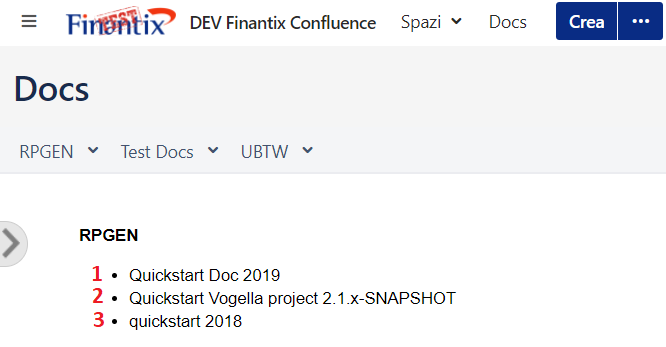
\includegraphics[width=0.7\textwidth]{immagini/DocsExamples.png}\\
		\caption{Screenshot di un esempio di Docs Plug-in}
	\end{figure}

% ---------------------------



\begin{figure}[H]
    \centering
    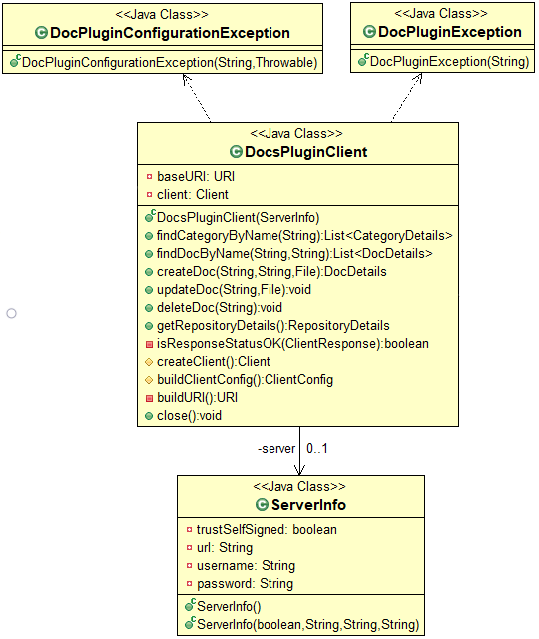
\includegraphics[width=0.9\textwidth]{immagini/client.png}\\
    \caption{Diagramma delle classi relativo al client}
\end{figure}

Il client è creato da AbstractPluginMojo ed è un oggetto di tipo \txt{DocsPluginClient}.
Questa classe fornisce tutto il necessario per creare ed usare un'istanza del client Jersey: riceve le informazioni per la configurazione da ServerInfo (un semplice Java bean simile a ServerBean) e produce la directory di base richiesta per svolgere qualunque tipo di chiamata REST.
I metodi che compiono delle chiamate REST sono:

\begin{table}[H]
    \begin{paddedtablex}[1.7]{\textwidth}{XcX}
        \rowcolor{beautyblue}\textbf{Nome} & \textbf{Richiesta} & \textbf{Descrizione} \\
        \toprule

        \txt{findCategoryByName(String categoryName)} & \bd{GET} & Ritorna una lista di categorie esistenti, il cui nome coincide con la stringa data \\
        \txt{findDocByName(String categoryId, String docName)} & \bd{GET}  & Ritorna una lista di doc esistenti all'interno di una categoria esistente e i cui nomi coincidono con la stringa data \\
        \txt{createDoc(String categoryId, String docName, File docArchive)} & \bd{PUT} & Crea la pagina doc all'interno di una categoria esistente, con l'archivio e il nome dato \\
        \txt{updateDoc(String docKey, File docArchive)} & \bd{POST} & Aggiorna la pagina doc identificata dalla \txt{docKey} data, con l'archivio dato \\
        \txt{getRepositoryDetails()} & \bd{GET} & Ritorna tutti i dettagli relativi alla repository: tutte le categorie e i doc esistenti \\
        \txt{deleteDoc(String docKey)} & \bd{DELETE} & Elimina la pgina doc relativa alla \txt{docKey} data \\

        \bottomrule
    \end{paddedtablex}
    \caption{Metodi di DocsPluginClient che compiono chiamate REST}
\end{table}

Molti di questi metodi possono tirare un'eccezione di tipo \txt{DocPluginException} quando la risposta del client ricevuta da Confluence in fase di comunicazione.

Un'altra eccezione che DocsPluginClient può tirare è \txt{DocPluginConfigurationException}: un'eccezione RuntimeException che può avvenire durante la creazione del client.



\begin{figure}[H]
    \centering
    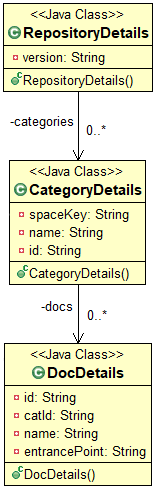
\includegraphics[width=0.25\textwidth]{immagini/details.png}\\
    \caption{Diagramma delle classi relativo ai dettagli di ogni componente del plugin Confluence}
\end{figure}

Inoltre è importante specificare che una chiamata REST, come per esempio una di quelle di tipo GET, ottiene le specifiche di una categoria o un \emph{doc} tramite un file JSON.
Questi JSON sono trasformati da JAXB in oggetti Java.
A questo scopo, sono state create le seguenti classi:
\begin{itemize}
    \item \txt{RepositoryDetails}: informazioni sulla repository (comprende a sua volta tutte le informazioni sulle categorie e i loro \emph{doc});
    \item \txt{CategoryDetails}: informazioni sulla categoria (comprende a sua volta tutti i \emph{doc} contenuti);
    \item \txt{DocDetails}: informazioni sulla pagina \emph{doc}.
\end{itemize}



    \subsection{Riepilogo delle classi}

    \begin{table}[H]
		\begin{paddedtablex}[1.7]{\textwidth}{cX}
			\rowcolor{beautyblue}\textbf{Nome} & \textbf{Breve descrizione} \\
			\toprule

			AbstractPluginMojo & Classe astratta dei mojo del plugin \\
            CleanupMojo & Classe mojo coincidente con il \emph{goal cleanup}: elimina la documentazione ``SNAPSHOT'' \\
            PublisherMojo & Classe mojo coincidente con il \emph{goal publish}: pubblica la documentazione software \\
            DocsPluginClient & Client del plugin che realizza chiamate REST \\
            RepositoryDetails & Oggetto Java che corrisponde al JSON riguardante i dettagli della repository \\
            CategoryDetails & Oggetto Java che corrisponde al JSON riguardante i dettagli di una categoria \\
            DocDetails & Oggetto Java che corrisponde al JSON riguardante i dettagli di un \emph{doc} \\
            ServerBean & Java bean contenente le informazioni del sever \\
            DocsPluginException & Eccezione sollevata da DocsPluginClient per la comunicazione con il server \\
            DocsPluginConfigurationException & RunTimeException sollevata da DocsPluginClient per problemi di configurazione \\

			\bottomrule
		\end{paddedtablex}
		\caption{Tabella riassuntiva delle classi}
	\end{table}



\section{Diagrammi di sequenza}
\label{sec:diagrammi-sequenza}

\subsection{Diagramma della pubblicazione della documentazione}
Ecco come funziona la pubblicazione della documentazione:

\begin{figure}[H]
    \centering
    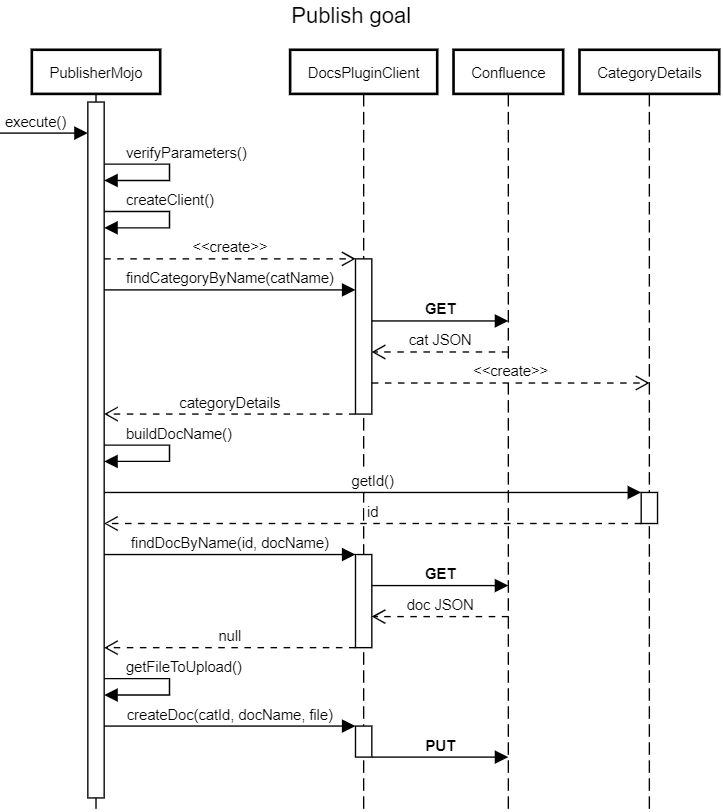
\includegraphics[width=\textwidth]{immagini/SeqPublish.png}\\
    % 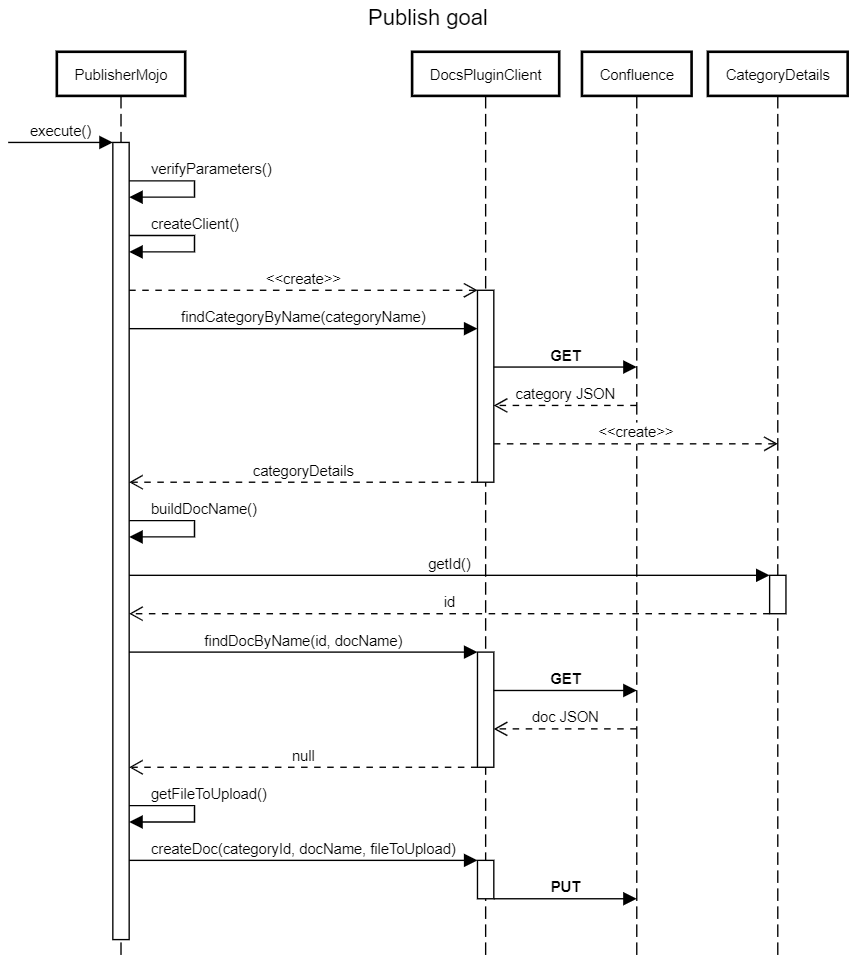
\includegraphics[width=\textwidth]{immagini/CreateDocSequence.png}\\
    \caption{Diagramma di sequenza relativo al \emph{goal publish}}
\end{figure}

Quando PublisherMojo viene eseguito, esso verifica la correttezza dei parametri dati e sospende l'esecuzione se necessario (per esempio se \txt{skip} è \txt{true}, ecc).

Dopo di che un'istanza di DocsPluginClient viene creata in modo da permettere le operazioni del client.
PublisherMojo usa DocsPluginClient per ricevere i dettagli della categoria appartenente al nome dato in fase di configurazione dall'utente.
Questo accade perché DocsPluginClient comunica con Confluence.
Il JSON che esso riceve da Confluence è trasformato nel relativo oggetto Java CategoryDetails.

Successivamente PublisherMojo costruisce il titolo della pagina \emph{doc} tramite nome e versione della documentazione.
In questo modo è possibile trovare il \emph{doc} con quel determinato titolo.
PublisherMojo ottiene l'id della categoria dall'oggetto precedentemente creato e richiede al client di trovare il \emph{doc} all'interno di quella categoria.

In questo caso, il JSON ritornato sarà vuoto perché la pagina \emph{doc} ancora non esiste.
A questo punto PublisherMojo ottiene l'archivio da pubblicare, che sarà l'archivio dato dall'utente o un nuovo archivio generato.

Infine la pagina \emph{doc} può essere creata all'interno della categoria con il nome e l'archivio selezionati. \\

L'aggiornamento di una pagina \emph{doc} funziona in maniera molto similare.
Le uniche differenze dallo scenario precedente si trovano dal JSON riguradante il \emph{doc} ritornato da Confluence in poi.
Esso non sarà vuoto, bensì conterrà le informazioni del \emph{doc} esistente.
A questo punto verrebbe chiamato un oggetto di tipo DocDeatails e il metodo \txt{udpateDoc()} verrebbe chiamato al posto di \txt{createDoc()}.


\subsection{Diagramma della pulizia della documentazione}

% \begin{figure}[H]
%     \centering
%     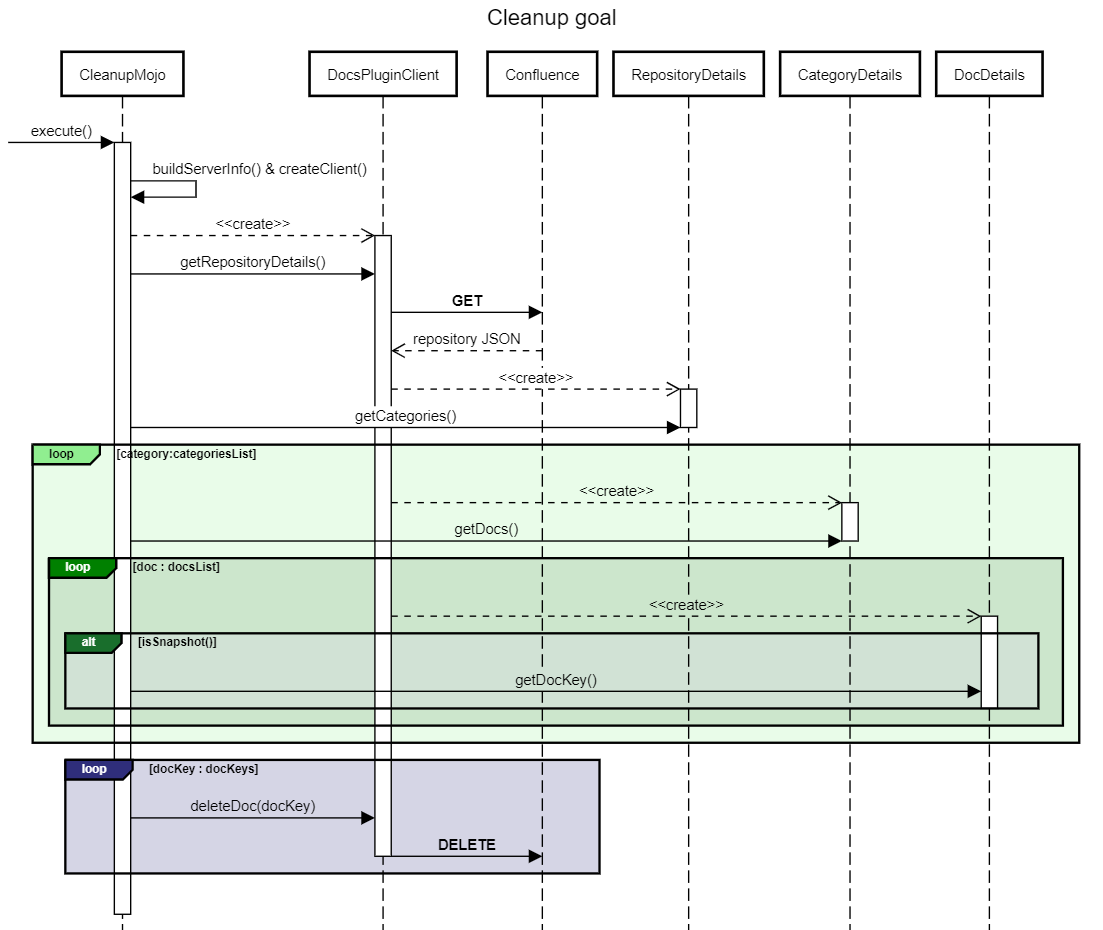
\includegraphics[width=\textwidth]{immagini/SequenceCleanupConfluence.png}\\
%     \caption{Diagramma di sequenza relativo al \emph{goal cleanup}}
% \end{figure}

\begin{figure}[H]
    \centering
    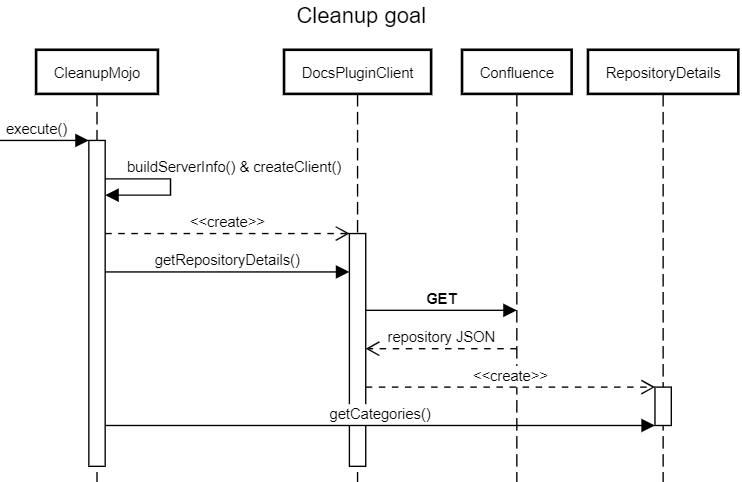
\includegraphics[width=\textwidth]{immagini/CleanupSeq1.png}\\
    \caption{Diagramma di sequenza relativo al \emph{goal cleanup} (1)}
\end{figure}

Prima di tutto, CleanupMojo agisce come PublisherMojo: crea un DocsPluginClient.
Grazie ad esso ottiene i dettagli relativi alla repository attraverso una chiamata GET a Confluence.
Il JSON ricevuto come risposta viene trasformato in un oggetto Java RepositoryDetails.
CleanupMojo ricava la lista di categorie dal RepositoryDetails precedentemente creato e itera su di esso.

\begin{figure}[H]
    \centering
    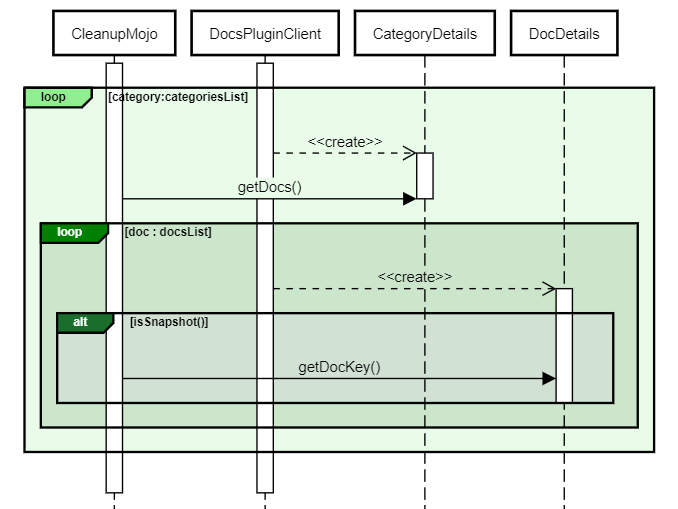
\includegraphics[width=\textwidth]{immagini/CleanupSeq2.png}\\
    \caption{Diagramma di sequenza relativo al \emph{goal cleanup} (2)}
\end{figure}

A questo punto richiede ad ogni CategoryDetails la sua lista di \emph{doc}.
Itera su ogni \emph{doc} controllandone il titolo per verificare se contiene ``SNAPSHOT''.
Se questa condizione è verificata, viene presa la chiave identificativa del \emph{doc} (\txt{docKey}).

\begin{figure}[H]
    \centering
    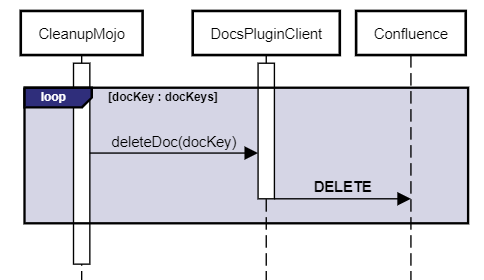
\includegraphics[width=0.7\textwidth]{immagini/CleanupSeq3.png}\\
    \caption{Diagramma di sequenza relativo al \emph{goal cleanup} (3)}
\end{figure}

Infine CleanupMojo elimina ogni pagina \emph{doc} all'interno del plugin Confluence \emph{Docs} di cui possiede l'identificativo.



%**************************************************************
% \section{Ciclo di vita del software}
% \label{sec:ciclo-vita-software}

%**************************************************************
% \section{Progettazione}
% \label{sec:progettazione}

% \subsubsection{Namespace 1} %**************************
% Descrizione namespace 1.

% \begin{namespacedesc}
%     \classdesc{Classe 1}{Descrizione classe 1}
%     \classdesc{Classe 2}{Descrizione classe 2}
% \end{namespacedesc}


%**************************************************************
\section{Design Pattern utilizzati}

\subsection{Template Method}

%**************************************************************
% \section{Codifica}
